\documentclass[a4paper,12pt,nottoc]{article}
\usepackage{graphicx}
\usepackage[left = 3cm, right = 2cm, top = 2cm, bottom = 2cm]{geometry}
\usepackage{makecell}
\usepackage{booktabs}
\usepackage[justification=centering]{caption}
\usepackage{listings}
\usepackage{color}
\usepackage{xcolor}
\usepackage{hyperref}
\usepackage{tocbibind}
\usepackage{amsmath}
\usepackage{siunitx}
\usepackage{mhchem}
\hypersetup{
    colorlinks=true,
    linkcolor=blue,
    filecolor=blue,      
    urlcolor=blue,
    citecolor=blue,
}

\begin{document}

\begin{center}{\LARGE Detecting Fake News with Supervised Learning}\\\vspace{.5cm}Benjamin R. Perucco\\\vspace{.25cm}December 30, 2020\end{center}

\section{Definition}

\subsection{Project Overview}

Our world is highly interconnected and it is of paramount importance that citizens are informed objectively about issues that influence and shape our world (like issues on geopolitics or climate change). The internet lead to a rise of news media (e.g. social media, news portals, etc.) to report on these stories. The vast amount of (online) articles available yield a new phenomenon called fake news. Fake news is false or misleading information presented as news and can reduce the impact of real news \cite{bib:fakenews}. 

\subsection{Problem Statement}

This works' intention is about answering the question whether machine learning can be applied to classify a news article as truthful or fake. There are several articles available where Ahmed et al. classified news articles \cite{bib:ahmed-2017} or hotel guest reviews \cite{bib:ahmed-2018} to be truthful or fake. Ahmed et al. used natural language processing (NLP) models to transform text into a structured, mathematical representation and achieved accuracies of 92\% \cite{bib:ahmed-2017}.\\

\noindent Based on a set of features $\{f_{1}, f_{2}, f_{3}, ... \}$ extracted from news articles, a machine learning algorithm needs to be trained to find the relationship $\hat{\theta}$ between the a priori known classifiction of the news articles $y$ ($=0$ for truthful and $=1$ for fake) and the set of extracted features $\{f_{1}, f_{2}, f_{3}, ... \}$. The relation can be written as

\begin{gather}
\hat{y} =\hat{\theta}(X)
\end{gather}

\noindent where $\hat{y}$ is the predicted class label by the trained function $\hat{\theta}$ applied to a feature matrix $X$. $\hat{\theta}$ must be trained on available data, such that

\begin{gather}\label{eq:sse}
\sum_{i=1}^{n} \left(y - \hat{y} \right)^2
\end{gather}

\noindent is minimal. Here it is assumed that we have $n$ news articles where it is already known whether they are truthful or not. A first step to be worked on in this report is to answer how to extract a feature matrix $X$ from a set of texts (or documents). How reliable is the prediction of class labels on unseen news articles once the function $\hat{\theta}$ has been found.

\subsection{Metrics}

Equation \ref{eq:sse} is rather used for regression problems where the predicted output is a continuous variable. For classification problems like news article classification into a truthful ($= 0$) and a fake class ($= 1$), the accuracy is a better metric. This can be nicely demonstrated by the confusion matrix

\begin{gather}
\begin{bmatrix}
& 1 & 0 \\
1 & \textrm{TP} & \textrm{FP} \\
0 & \textrm{FN} & \textrm{TN}
\end{bmatrix}.
\end{gather}

\noindent The entries in the row indicate predicted classes and the entries in the columns represent the real classes. Furthermore, TP stands for true positives, TN for true negatives, FP for false positives and FN for false negatives. To asses the performance of $\hat{\theta}$, the accuracy $a$ is considered, which can be calculated as

\begin{gather}\label{eq:acc}
a = \frac{\textrm{TP} + \textrm{TN}}{\textrm{TP} + \textrm{TN} + \textrm{FN} + \textrm{FP}}.
\end{gather}

\section{Analysis}

\subsection{Algorithms and Techniques}

News articles must be converted into a structured, mathematical representation in order it can be used by machine learning techniques. The following chapters disucss how we can convert text into numerical features.

\subsubsection{n-gram Model}

The $n$-gram is usually defined a contiguous sequence of words with length $n$. For example, if $n = 1$, we speak of a unigram that contains only single word tokens. Or if $n = 2$, we denote this as a bigram which is built on two adjacent word tokens.\\

\noindent Consider the following text: ``Sometimes we eat green apples, and sometimes, the apples we eat are red.'' Based on a unigram (1-gram), we obtain a set of tokens: $\{$'sometimes', `we', `eat', `apples', `green', `and', `the', `are', `red'$\}$. We can derive a frequency array of tokens in the text: [2, 2, 2, 2, 1, 1, 1, 1, 1]. For the bigram (2-gram), another set of tokens is obtained: $\{$'sometimes we', `we eat', `eat green', `green apples', `apples and', `and sometimes', `sometimes the', `the apples', `apples we', `eat are', `are red'$\}$. The corresponding frequency array of tokens in the text is: [1, 1, 1, 1, 1, 1, 1, 1, 1, 1, 1]. Please note that punctuation is not considered when converting text into tokens.\\

\noindent In order to build frequency arrays for a set of texts (or documents), a common vocabulary needs to be built of which the $n$-gram model is underlying principle.

\subsubsection{Vocabulary}

Consider a corpus $D$ which contains a set of documents $\{d_1, d_2, d_3, ..., d_n\}$. Then a vocubulary $F$ is a set of tokens $\{f_1, f_2, f_3, ..., f_m\}$ extracted from the corpus $D$. Please remind yourself that a token is created based on the $n$-gram model. Usually for a set of tokens, only the $m$ mostly occuring tokens in a corpus $D$ are considered. In the following, the tokens are denoted as features as these construct the features (or independent variables) of a machine learning model.\\

\subsubsection{Definitions}

Let $\sigma(d_i, f_j)$ denote the number of occurances of feature $f_j$ in document $d_i$. Then a feature matrix $S$ can be built, where

\begin{gather}
S =
\begin{bmatrix}
\sigma(d_1, f_1) & \sigma(d_1, f_2) & \sigma(d_1, f_3) & ... & \sigma(d_1, f_m) \\
\sigma(d_2, f_1) & \sigma(d_2, f_2) & \sigma(d_2, f_3) & ... & \sigma(d_2, f_m) \\
\sigma(d_3, f_1) & \sigma(d_3, f_2) & \sigma(d_3, f_3) & ... & \sigma(d_3, f_m) \\
... & ... & ... & ... & ... & \\
 \sigma(d_n, f_1) & \sigma(d_n, f_2) & \sigma(d_n, f_3) & ... & \sigma(d_n, f_m)
\end{bmatrix}.
\end{gather}

\noindent An element $\sigma(d_i, f_j)$ in matrix $S$ (representing the document $d_i$ and feature $f_j$) is abbreviated using the notation $\sigma_{ij}$ for simplicity.

\subsubsection{Term Frequency Model}

The matrix $S$ could be already used for machine learning. Features usually need to be normalized in machine learning to increase performance. Therefore, the term frequency (TF) model normalizes matrix $S$ leading to matrix $\hat{S}$. An element $\hat{\sigma}_{ij}$ of matrix $\hat{S}$ is written as

\begin{gather}\label{eq:tf}
\hat{\sigma}_{ij} = \frac{\sigma_{ij}}{\sum_{j=1}^{m}\sigma_{ij}}.
\end{gather}

\noindent Or spoken in plain language: the number of occurances of a token $f_j$ in a document $d_i$ is divided by the total number of occurances of all tokens $\{f_1, f_2, f_3, ..., f_m\}$ in the same document $d_i$. So we end up with a representation where the importance of each feature can be compared to other features in the same document.

\subsubsection{Inverse Document Frequency Model}

The inverse document frequency (IDF) model is used to define the feature importance not just in a document $d_i$ but also compare its importance within a corpus $D$. A matrix $E$ is introduced, where an element $\epsilon_{ij}$ of matrix $E$ is $1$ if $\hat{\sigma}_{ij} > 0$ (or $\sigma_{ij} > 0$). An inverse normalization is applied to the matrix $E$ resulting in a vector $\hat{e}$. An element $\hat{\epsilon}_{j}$ of vector $\hat{e}$ is calculated as

\begin{gather}\label{eq:idf}
\hat{\epsilon}_{j} = 1 + \textrm{log}\left[\frac{|D|}{\sum_{i=1}^{n}\epsilon_{ij}}\right].
\end{gather}

\noindent Or spoken in plain language: in a corpus $D$ which comprises of a set of documents $\{d_1, d_2, d_3, ..., d_n\}$, it is counted in how many documents the feature $f_j$ appears. This number is used to divide the number of documents $|D|$ in a corpus $D$. Consider two examples: if a feature $f_j$ occurs in each document $\{d_1, d_2, d_3, ..., d_n\}$, we divide the number of documents $|D|$ in a corpus $D$ by the same number. So equation \ref{eq:idf} results in $1$, weighting feature $f_j$ as $1$. On the other hand, if a feature $f_j$ occurs only in one document, equation \ref{eq:idf} produces a much larger number, thus increasing the weight of feature $f_j$ in the corpus $D$.\\

\noindent Finally, a matrix $\hat{P}$ is obtained as the element-wise product of the term frequency matrix $\hat{S}$ and the inverse document frequency vector $\hat{e}$, written as $\hat{P} = \hat{S} \odot \hat{e}$. For an element $\hat{\pi}_{ij}$ of matrix $\hat{P}$, this is written as

\begin{gather}\label{eq:tf-idf}
\hat{\pi}_{ij} = \hat{\sigma}_{ij} \cdot \hat{\epsilon}_{j},\;\;\textrm{element-wise for}\;j = 1, 2, 3, ..., m .
\end{gather}

\noindent This term is denoted as the term frequency inverse document frequency model (TF-IDF).

\subsection{Data Exploration}

A set of truthful and fake news articles is available on kaggle.com \cite{bib:kaggle}. The data was collected from real world sources. Truthful articles were obtained from Reuters and fake news articles were gathered from unreliable websites that were flagged by Politifact which is a fact-checking organization. These datasets contain different types of articles on different topics, the majority of articles focus on political and world news topics \cite{bib:ahmed-2018}.\\

\noindent There are 44,898 articles in total in the corpus. 21,417 of the articles are classified as truthful and 23,481 are classified as fake, so both class labels are roughly balanced. Approximately 6,169 of the articles are not unique. The duplicates are being removed after text processing discussed in chapter \ref{chap:data-preproc}.

\subsubsection{Visual Analysis of Top Features}

A first glimpse of the top 20 unigrams per class is given in figure \ref{fig:top20}. Please note that the extracted unigrams are based on the processed text. It can be observed from the unigrams that probably the most discussed topic in the set of news articles is the presidential election in the U.S. during the year 2016. Despite some unigrams that are used frequently in both classes of articles (like said, trump, presid, republican, etc.), we also see distinct unigrams only used in one class of articles.

\begin{figure}[h]
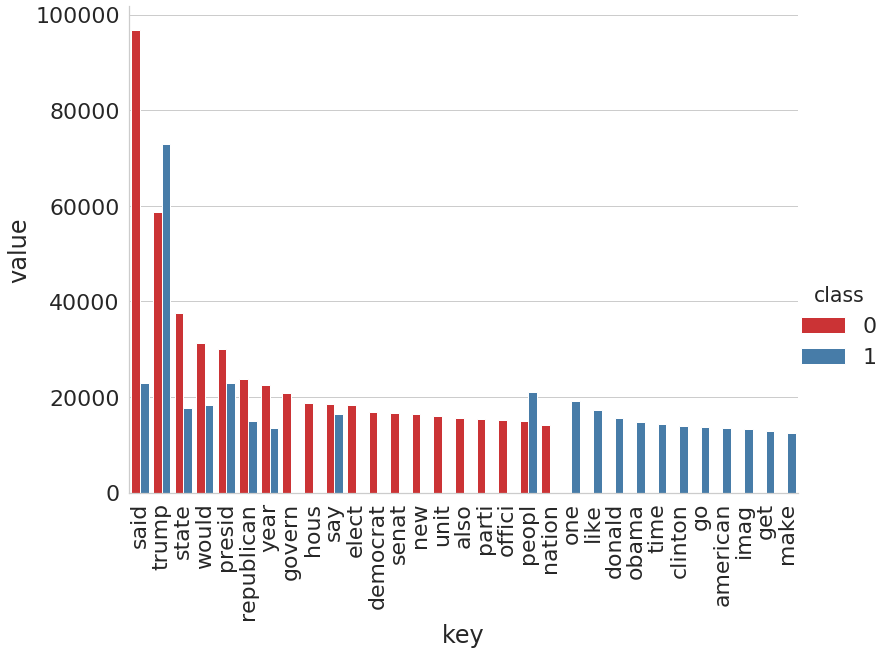
\includegraphics[width=14cm]{output/word_analysis_1.png}
\centering
\caption{Frequency of the top 20 unigrams per class extracted from the corpus.}\label{fig:top20}
\end{figure}

\section{Methodology}

\subsection{Data Preprocessing}\label{chap:data-preproc}

Raw text has to be brought into a clean state in order for feature extraction. Several text cleansing steps are performed like removal of introductory statements, dates, hyperlinks, numbers and stopwords. Finally, so called stemming is performed to end up with the stem of a word (for example cat should identify such strings as cats, catlike, and catty \cite{bib:stemming}).

\subsection{Implementation}

\subsubsection{Feature Extraction Method}

Then the randomized corpus is split into three different datasets as displayed in the table \ref{tab:datapreproc} below.

\begin{table}[h]
\begin{center}
\begin{tabular}{| l | l | r | c | c | c |}
\hline
Name & Purpose & Size & TF & IDF & TF-IDF \\
\hline
Training & Model training & 60\% & $\hat{S}_{\textrm{train}}$ & $\hat{E}_{\textrm{train}}$ & $\hat{S}_{\textrm{train}} \odot \hat{E}_{\textrm{train}}$ \\  
Test & Hyperparameter tuning & 20\% & $\hat{S}_{\textrm{test}}$ & $\hat{E}_{\textrm{train}}$ & $\hat{S}_{\textrm{test}} \odot \hat{E}_{\textrm{train}}$ \\    
Validation & Model validation & 20\% & $\hat{S}_{\textrm{valid}}$ & $\hat{E}_{\textrm{train}}$ & $\hat{S}_{\textrm{valid}} \odot \hat{E}_{\textrm{train}}$ \\
\hline 
\end{tabular}
\end{center}
\caption{Data preprocessing and feature extraction methods applied.}\label{tab:datapreproc}
\end{table}

\noindent It is good practise not to use the same data for model training and validation. For hyperparameter tuning a test dataset is used to avoid overfitting.\\

\noindent Term frequency (TF) feature matrices are calculated for each set according to equation \ref{eq:tf}. In comparison, the inverse document frequency (IDF) feature matrix is only calculated for the training set according to equation \ref{eq:idf}. The reason is that the validation and test set should simulate the performance behaviour in case of new unseen data. Therefore,  the IDF feature matrix is estimated on a hypothetical training set and the resulting matrix $\hat{E}_{\textrm{train}}$ is used for the transformation of all sets into the TF-IDF feature space according to equation \ref{eq:tf-idf}. Contrary, the TF feature matrix describes the relative importance of features in a single document. This is independent of other documents in the corpus and therefore, we can derive three matrices $\hat{S}_{\textrm{train}}$, $\hat{S}_{\textrm{test}}$ and $\hat{S}_{\textrm{valid}}$ for the three sets.

\subsubsection{Modeling}

\noindent SageMaker \cite{bib:sagemaker} is used as the training and deployment platform for the machine learning models. The evaluated machine learning models are based on the sci-kit learn framework \cite{bib:scikit-learn} because of its simplicity to try out different machine learning models.\\

\noindent The following models k nearest neighbor (knn), support vector machine (svm), logistic regression (log), gradient boosting (gbc) and multilayer perceptron (mlp) are used. Furthermore, the TF and TF-IDF feature extraction methods are applied. The feature size is set to 500, 1,000 and 5,000 features and unigram and bigram are used for feature extraction.

\subsection{Refinement}

Hyperparameter tuning is performed on the training set and tested on the test set according to the accuracy (equation \ref{eq:acc}). A hyperparameter set is search for which maximizes the accuracy. For the hyperparameter search, 20 combinations are evaluted and in total this results in 1,200 models to be trained and tested (5 models x 2 feature extraction methods x 3 different feature sizes x 2 differnt $n$-grams x 20 models for hyperparameter tuning). In the following table \ref{tab:hyperparam}, the model hyperparameters as well as its varied ranges are shown. 

\begin{table}[h]
\begin{center}
\begin{tabular}{| l | c | l |}
\hline
Parameter & Type & Range \\
\hline
\multicolumn{3}{| c |}{k nearest neighbor \cite{bib:knn}} \\ [.1cm]
\hline
n neighbors & int & [3, 15] \\
weight & cat & 'uniform', 'distance'\\
p & int & [1, 8] \\
\hline 
\multicolumn{3}{| c |}{support vector machine \cite{bib:svm}} \\ [.1cm]
\hline
random state & int & 1 \\
kernel & cat & `poly' \\
C & float & [0.001, 3.0] \\
degree & int & [2, 3] \\
\hline 
\multicolumn{3}{| c |}{logistic regression \cite{bib:log}} \\ [.1cm]
\hline
max iter & int & 10,000 \\
C & float & [0.001, 3.0] \\
\hline
\multicolumn{3}{| c |}{gradient boosting \cite{bib:gbc}} \\ [.1cm]
\hline
random state & int & 1	 \\
learning rate & float & [0.001, 0.5] \\
n estimators & int & [100, 1,000] \\
max depth & int & [2, 10] \\
\hline 
\multicolumn{3}{| c |}{multilayer perceptron \cite{bib:mlp}} \\ [.1cm]
\hline
random state & int & 1	 \\
learning rate & float & [0.0001, 0.1] \\
max iter & int & [100, 10,000] \\
activation & cat & 'identity', 'logistic', 'relu', 'tanh' \\
hidden layer size & int & [2, 10] \\
start size$^\textrm{1}$ & int & [10, 1,000] \\
end size$^\textrm{1}$ & int & [10, 1,000] \\
\hline
\end{tabular}
\caption{$^\textrm{1}$ Note that start and end size are not available as parameters in the multilayer perceptron model in scikit-learn. Based on the hidden layer size and its start and end size, a linear interpoliation is performed for the number of neurons in between in case the hidden layer size is higher than 2.}\label{tab:hyperparam}
\end{center}
\end{table}

\clearpage
\section{Results}

\subsection{Model Evaluation and Validation}

\subsubsection{Influence of Parameter Variation}

There are 60 parameter variations studied in total using hyperparameter tuning in SageMaker \cite{bib:sagemaker} (5 models x 2 feature extraction methods x 3 different feature sizes x 2 different $n$-grams). The influence of the different parameters is demonstrated below in figure \ref{fig:influenceparams}.

\begin{figure}[h]
\begin{center}
\begin{tabular}{c c}
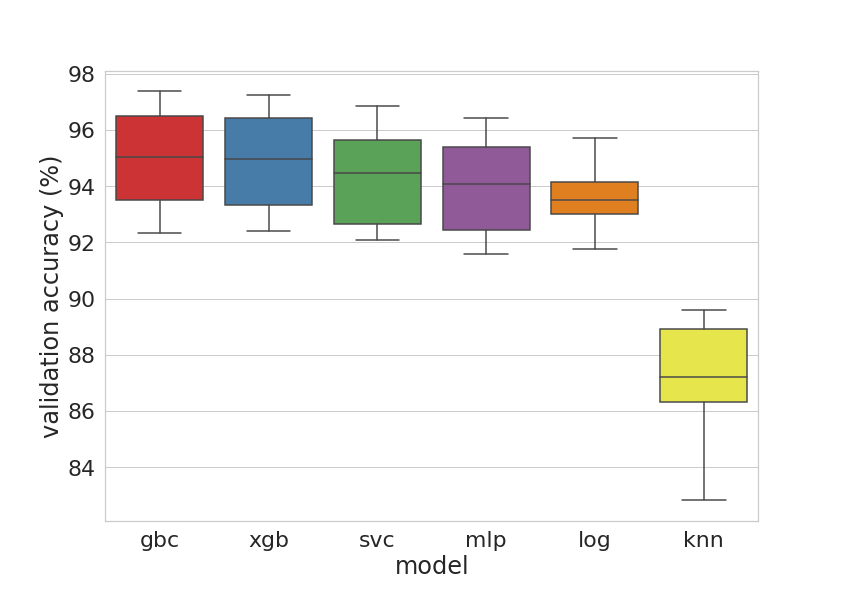
\includegraphics[width=8cm]{output/model_performance.png} & 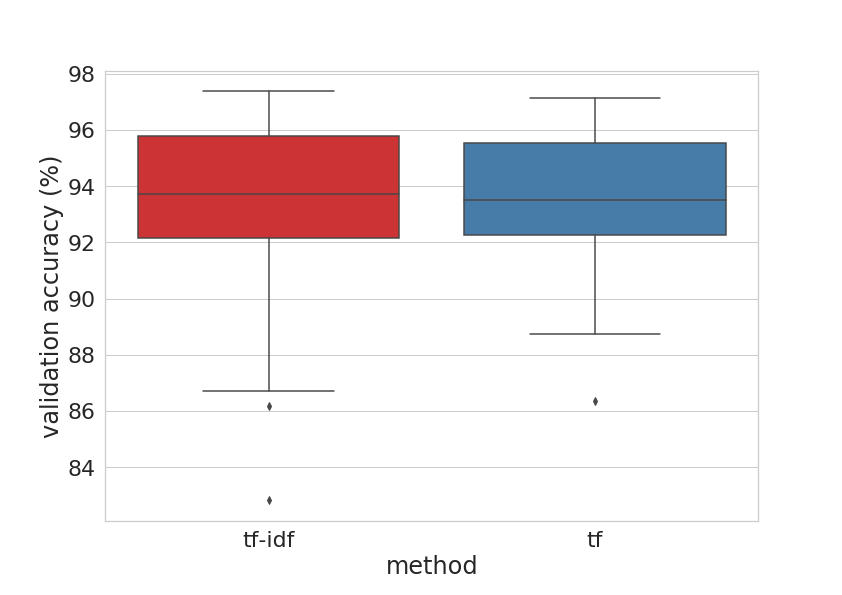
\includegraphics[width=8cm]{output/method_performance.png} \\
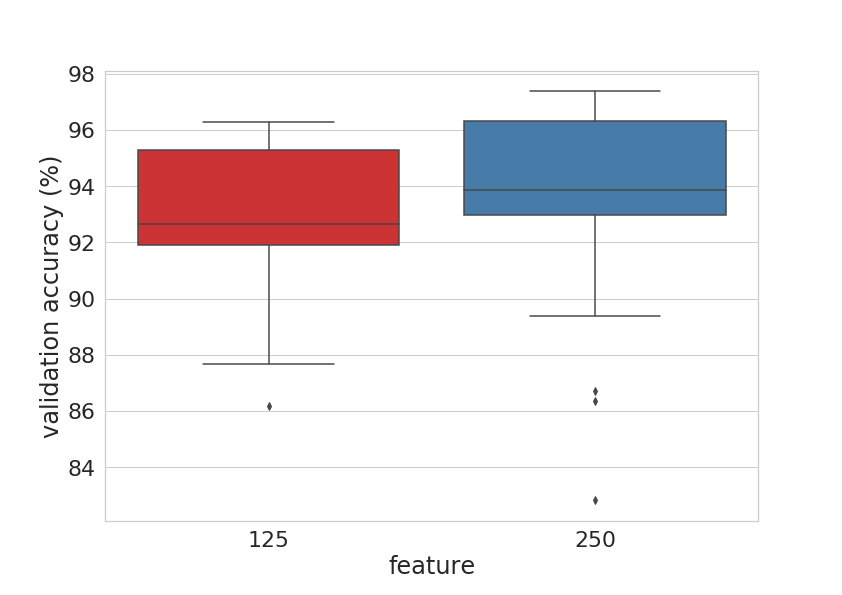
\includegraphics[width=8cm]{output/feature_performance.png} & 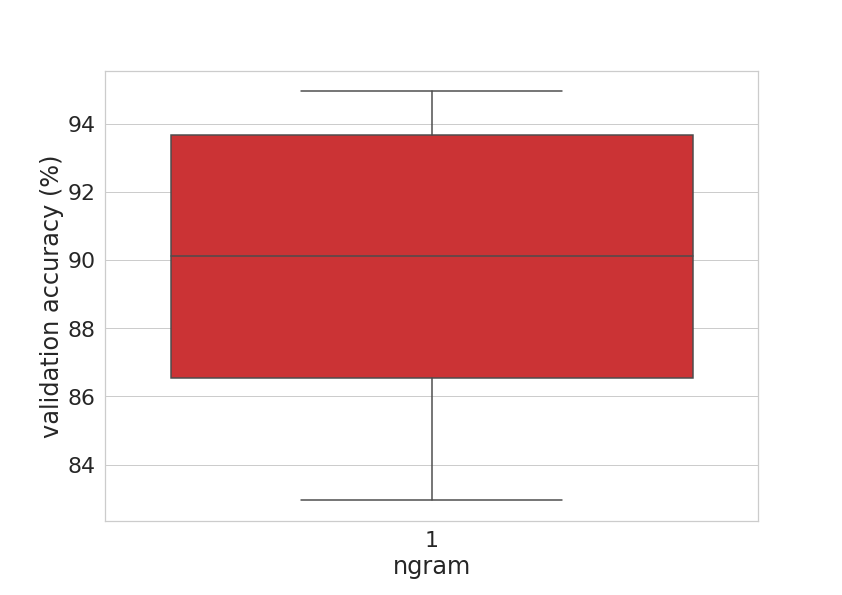
\includegraphics[width=8cm]{output/ngram_performance.png} \\
\end{tabular}
\end{center}
\caption{The influence on the accuracy of varied models, feature extraction methods, feature sizes and different $n$-grams is demonstrated.}\label{fig:influenceparams}
\end{figure}

\subsubsection{Accuracy Performances}

The parameter combinations leading in the best five accuracy performances are shown in the table \ref{tab:accperf} below.

\begin{table}[h]
\begin{center}
\begin{tabular}{| l | l | c | c | c | c |}
\hline
Model & Method & Feature & $n$-gram & \thead{Accuracy on \\ test set (\%)} & \thead{Accuracy on \\ validation set (\%)} \\
\hline
knn & TF & 5,000 & 1 & 94.83 & 94.94 \\
knn & TF-IDF & 1,000 & 1 & 93.96 & 94.20 \\
knn & TF-IDF & 5,000 & 1 & 91.27 & 92.07	 \\
\hline 
\end{tabular}
\end{center}
\caption{Parameter combinations leading in the best three accuracies.}\label{tab:accperf}
\end{table}

\subsubsection{Detailed Results}

Detailed results on achieved accuracies, model hyperparameters and other varied parameters can be found on the \href{https://github.com/benjaminperucco/udacity-nano-mle/blob/master/5%20Capstone/2%20Project/3_postprocessing.ipynb}{Github repository}. 

\subsection{Justification}




\section{Conclusion}

\subsection{Reflection}\label{chap:reflection}

Machine learning models are able to classify articles into two classes of truthful and fake articles really well. It can be shown that accuracies of 97\% can be achieved. But one has to ask the question what has been the methodology to decide which article is fake and which article is truthful. For example all truthful articles are from Reuters and fake articles were classified by Politifact. Even though this methodology has been consistent for the set of articles analyzed in this work, it does not necessarily mean that new and unseen articles from other sources can be classified equally well by a machine learning model. In my opinion this is one of the remaining question mark and needs to be answered.

\subsection{Improvement}

Further investigations can be done in order to achieve an even better classifiction, or increase training and prediction computation speed:

\begin{itemize}
\item{With such a large corpus of 44,898 documents, it can be difficult to achieve a text processing that is clean from text not related to the article (hyperlinks, references to twitter accounts, etc.). A second thorough investigation must dive deeper into the news articles to remove any unwanted stuff that remained from the current text processing.}
\item{The methodology of article classification has to be reviewed and one has to clarify how well the classification performs on completely different sources of news articles (as mentioned in chapter \ref{chap:reflection}).}
\item{Using a feature size of 5,000 leads to long training computation time. Calculating the correlation between the individual features and focussing on features with low correlation can help to reduce computation cost. Another option is to apply principal component analysis to reduce the number of features.}
\item{No built-in algorithms of SageMaker \cite{bib:sagemaker}, such as XGBoost, are taken into account so far. These algorithms may improve accuracy as well as increse computation speed because they have been optimized by Amazon to handle large datasets.}
\end{itemize}

\clearpage
\begin{thebibliography}{9}
\bibitem{bib:fakenews} Fake news, December 30, 2020, wikipedia.org, \\\href{https://en.wikipedia.org/wiki/Fake_news}{\texttt{https://en.wikipedia.org/wiki/Fake\_news}}
\bibitem{bib:ahmed-2017} Ahmed H., Traore I., Saad S. (2017) Detection of Online Fake News Using N-Gram Analysis and Machine Learning Techniques. In: Traore I., Woungang I., Awad A. (eds) Intelligent, Secure, and Dependable Systems in Distributed and Cloud Environments. ISDDC 2017. Lecture Notes in Computer Science, vol 10618. Springer, Cham. \\\href{https://doi.org/10.1007/978-3-319-69155-8_9}{\texttt{https://doi.org/10.1007/978-3-319-69155-8\_9}}
\bibitem{bib:ahmed-2018} Ahmed, H, Traore, I, Saad, S. Detecting opinion spams and fake news using text classification, Security and Privacy, 2018, \\\href{https://doi.org/10.1001/spy2.9}{\texttt{https://doi.org/10.1001/spy2.9}}
\bibitem{bib:kaggle} Fake and real news dataset, December 30, 2020, kaggle.com, \\\href{https://www.kaggle.com/clmentbisaillon/fake-and-real-news-dataset}{\texttt{https://www.kaggle.com/clmentbisaillon/fake-and-real-news-dataset}}
\bibitem{bib:stemming} Stemming, December 30, 2020, wikipedia.org, \\\href{https://en.wikipedia.org/wiki/Stemming}{\texttt{https://en.wikipedia.org/wiki/Stemming}}
\bibitem{bib:sagemaker} Amazon SageMaker, December 30, 2020, amazon.com, \\\href{https://aws.amazon.com/sagemaker}{\texttt{https://aws.amazon.com/sagemaker}}
\bibitem{bib:scikit-learn} scikit-learn - machine learning in Python, December 30, 2020, scikit-learn.org, \\\href{https://scikit-learn.org/stable}{\texttt{https://scikit-learn.org/stable}}
\bibitem{bib:knn} scikit-learn - k-nearest neighbors vote classifier, December 30, 2020, scikit-learn.org, \\\href{https://scikit-learn.org/stable/modules/generated/sklearn.neighbors.KNeighborsClassifier.html}{\texttt{https://scikit-learn.org/stable/modules/generated/\\sklearn.neighbors.KNeighborsClassifier.html}}
\bibitem{bib:svm} scikit-learn - c-support vector classification, December 30, 2020, scikit-learn.org, \\\href{https://scikit-learn.org/stable/modules/generated/sklearn.svm.SVC.html}{\texttt{https://scikit-learn.org/stable/modules/generated/\\sklearn.svm.SVC.html}}
\bibitem{bib:log} scikit-learn - logistic regression classifier, December 30, 2020, scikit-learn.org, \\\href{https://scikit-learn.org/stable/modules/generated/sklearn.linear_model.LogisticRegression.html}{\texttt{https://scikit-learn.org/stable/modules/generated/\\sklearn.linear\_model.LogisticRegression.html}}
\bibitem{bib:gbc} scikit-learn - gradient boosting for classification, December 30, 2020, scikit-learn.org, \\\href{https://scikit-learn.org/stable/modules/generated/sklearn.ensemble.GradientBoostingClassifier.html}{\texttt{https://scikit-learn.org/stable/modules/generated/\\sklearn.ensemble.GradientBoostingClassifier.html}}
\bibitem{bib:mlp} scikit-learn - multilayer perceptron classifier, December 30, 2020, scikit-learn.org, \\\href{https://scikit-learn.org/stable/modules/generated/sklearn.neural_network.MLPClassifier.html}{\texttt{https://scikit-learn.org/stable/modules/generated/\\sklearn.neural\_network.MLPClassifier.html}}
\end{thebibliography}

\end{document}